\chapter{\textit{TypeShield} Overview}
\label{chapter:TypeShild Overview}
We now provide a short overview of the made assumptions and the threat model in Section \ref{Adversary Model}. After this we give a highlevel overview of the ideas of parameter count and type based classification in Section \ref{Invariants for Targets and Callsites}. Finally, Section \ref{TypeShild Impact on COOP} describes the impact of our tool against the COOP exploit.

\section{Adversary Model and Assumptions}
\label{Adversary Model}
We largely use the same threat model and the same basic assumptions as described in the TypeArmor paper \cite{veen:typearmor}, meaning that our attacker has read and write access to the data sections of the attacked binary.  We also assume that the protected binary does not contain selfmodifying code, handcrafted assembly or any kind of obfuscation. We also consider pages to be either writeable or executable but not both at the same time. Furthermore we assume that our attacker has the ability to execute a memory corruption to hijack the programs control flow. As our schema targets only forward control flow, namely indirect function calls, we assume that a solution for backward CFI edges is in place.


\section{Invariants for Targets and Callsites}
\label{Invariants for Targets and Callsites}
Advanced code reuse attacks attempt to change the calltargets that are invoked within indirect callsites, standard CFI solutions cannot defend against this and TypeArmor proposed the approach of creating two sets of invariants. 

\begin{enumerate}
\item Indirect callsites provide a number of parameters (possibly overestimated compared to source)
\item Calltargets require a minimum number of parameters (possibly underestimated compared to source)
\end{enumerate}

The main idea is now that a callsite might not call any function in the binary but only calltargets that do not require more parameters than provided by the callsite itself. To achieve this classification of calltargets and callsites, TypeArmor proposed to use a modified version of forward liveness analysis for calltargets and backward reaching defintions analysis for callsites.


\section{\textit{TypeShield} Impact on COOP}
\label{TypeShild Impact on COOP}
The problem with relying solely on the parameter count is that a callsite being classified as using 6 or more parameters can use basically all address taken functions within the binary. This is however counterproductive and we attempt a possible solution, by extending the classification schema to the single parameters themselves:

\begin{enumerate}
\item Indirect callsites provides a maximum wideness of value to each parameter (possibly overestimated compared to source)
\item Calltargets require a minimum widness of value for each parameter(possibly underestimated compared to source)
\end{enumerate}

Basically the principle stays the same, but instead of just requiring that the callsite parameter count is not lower than the calltarget parameter count we now require the same also for the wideness of each parameter.

While there are still occurrences where callsites may target all calltargets, we split the buckets up into smaller ones, as shown in Figure \ref{fig:lattice3264}. For example in the paramcount oriented schema a callsite classified as (32,32) would be able to call functions classified as (64,0), however in the parameter wideness oriented schema that is not possible.

\begin{figure}[!h]
\centering
\resizebox{0.5\textwidth}{!}{
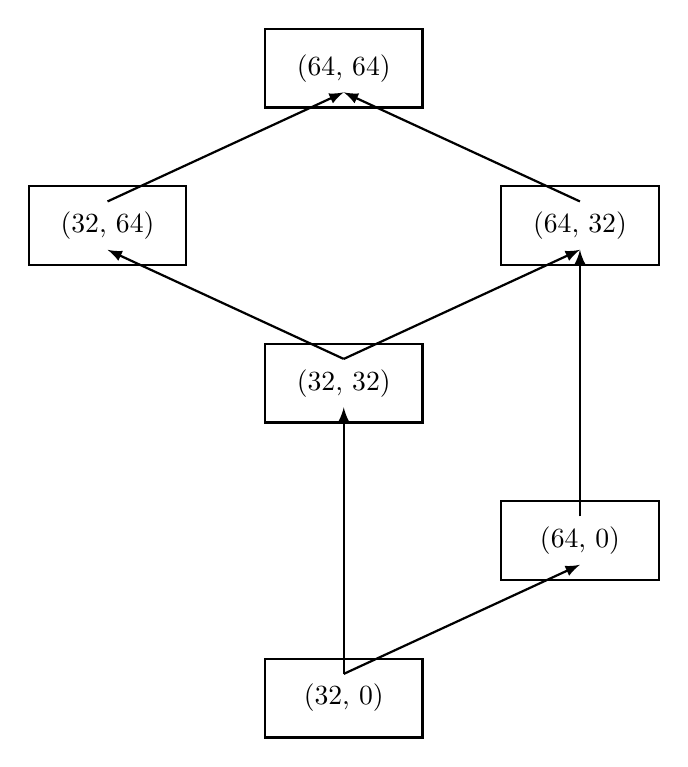
\begin{tikzpicture}


\draw[thick] (0,0) rectangle node[anchor=center]  (320) {(32, 0)} (2,-1);

\draw[thick] (3,2) rectangle node[anchor=center](640) {(64, 0)} (5,1);

\draw[thick] (0,3) rectangle node[anchor=center] (3232) {(32, 32)} (2,4);

\draw[thick] (3,5) rectangle node[anchor=center]  (6432) {(64, 32)} (5,6);
\draw[thick] (-1,5) rectangle node[anchor=center]  (3264)  {(32, 64)}(-3,6);

\draw[thick] (0,7) rectangle node[anchor=center](6464)   {(64, 64)} (2,8);

  \draw[draw, -latex, thick] (3264.north) -- (6464.south);
  \draw[draw, -latex, thick] (6432.north) -- (6464.south);
  \draw[draw, -latex, thick] (3232.north) -- (3264.south);
  \draw[draw, -latex, thick] (3232.north) -- (6432.south);
  
  \draw[draw, -latex, thick] (640.north) -- (6432.south);
  \draw[draw, -latex, thick] (320.north) -- (3232.south);
  \draw[draw, -latex, thick] (320.north) -- (640.south);
  
\end{tikzpicture}
}
\caption{Example for the wideness based schema when only using a parameter wideness of 64, 32 and 0 bits.}
\label{fig:lattice3264}
\end{figure}